\section{Подходы к эффективной реализации алгоритмов \label{implementation}}
Для реализации численных методов решения уравнения теплопроводности \eqref{eq:heat_equation_intro} и системы функционала плотности \eqref{eq:dhd_system_intro} был выбран язык программирования Python 3 \cite{Python3}. Выбор этого языка связан с простотой написания и внесения изменений в код, а так же богатая экосистема вокруг него. При использовании возможностей библиотек трехмерный расчет становится достаточно быстрым для проведения исследований. Перечислим, какими библиотеками мы воспользовались:
\begin{itemize}
\item Арифметические операции для массивов, заранее скомпилированные в машинный код, из библиотеки Numpy \cite{Numpy}
\item Компиляция во время исполнения отдельных участков кода с помощью библиотеки Numba \cite{Numba}
\item Некоторые алгоритмы линейной алгебры из библиотеки Scipy \cite{Scipy}
\end{itemize}

С помощью данных подходов мы избавляемся от большого количества циклов и оперируем векторами и матрицами более абстрактно.

\subsection{Символьная математика \label{implementation:symbolic}}
В исследуемых задачах теплопроводности \eqref{eq:heat_equation_intro} и функционала плотности \eqref{eq:dhd_system_intro} все функции, заданные аналитически, считаются гладкими. В данной работе мы много раз сталкивались и еще столкнемся с необходимостью посчитать аналитический вид частных производных:
\begin{enumerate}
    \item для функций, используемых в системе функционала плотности из обобщенной свободной энергии
    \item для вычисления матрицы Якоби или ее действия в безматричном подходе (раздел \ref{methods:computing_jacobi})
    \item для тестирования при восстановлении задачи из известного решения (раздел \ref{implementation:convergence})
\end{enumerate}

Формулы, которые мы дифференцируем, могут быть очень сложными, и их реализация в коде приводила бы к ошибкам. Процесс аналитического дифференцирования можно автоматизировать. В данной работе используется библиотека Sympy \cite{Sympy}. Создаются объекты, представляющие математические переменные. Исходные формулы выражаются через них аналитически в коде. После этого библиотека может найти определенные частные производные. Затем эти производные арифметически упрощаются. Из них может быть сгенерирован код на Python 3 с использованием библиотеки Numpy. Кроме того, можно получить код формул на языке C для дальнейшей компиляции. Этот подход используется в разделе \ref{implementation:cuda}.
\subsection{Использование CUDA \label{implementation:cuda}}
В дальнейшем планируется реализовать численный метод для неявного моделирования системы функционала плотности в декартовых координатах в 3D. Такой расчет должен быть высокопроизводительным, так как размеры решаемой линейной системы увеличатся кубически по сравнению с одномерной задачей. Оптимизации такого расчета на Python будет недостаточно. 
\par
Для многократного ускорения расчета можно перенести вычисления на GPU с помощью технологии CUDA \cite{Cuda}. Этот подход требует написания низкоуровневого кода на языке C\texttt{++}. Так, нам приходится выбирать между удобством реализации и производительностью. 
\par
Среди преимуществ высокоуровневой реализации отдельно выделим использование символьной математики. В системе функционала плотности физическая модель конкретных жидкостей задается с помощью свободной энергии $f(n_i)$ из формулы \eqref{eq:chemical_potential_intro}. Для моделей, применяемых на практике, это обычно сложная формула. Для расчета такой модели по методу функционала плотности понадобится найти аналитически производные этой функции по $n_i$. Для неявного метода в матрице Якоби понадобятся еще и вторые производные. Поэтому внедрение новых физических моделей в программу может быть очень трудозатратным. С помощью символьной математики этот процесс можно автоматизировать. При этом нельзя жертвовать скоростью расчета.
\par
Рассмотрим, как можно совместить преимущества символьной математики с разработкой эффективного кода с помощью библиотеки PyCuda \cite{Pycuda}. Алгоритм схематично изображен на рис. \ref{fig:cuda_architecture}.
Процесс, запускаемый с CPU на GPU, в рамках терминов CUDA принято называть \textit{ядром}. PyCuda позволяет запускать ядра CUDA из Python. Воспользуемся Sympy для генерации кода на С и добавим нужные атрибуты для компилятора CUDA. Так можно автоматически генерировать код, зависящий от физической модели, и связывать его с общим кодом для всей численной схемы.
Другим преимуществом PyCuda является автоматизированное управление указателями на массивы, находящиеся на GPU. Это избавляет от необходимости управлять памятью вручную. 
\par
Вызовы ядра CUDA происходят из Python с помощью PyCuda. Этот подход позволяет разделить низкоуровневый код численной схемы и вспомогательные задачи, от которых не требуется высокой производительности. Код для CUDA генерируется и компилируется из Python один раз, поэтому не замедляет расчет. 
При этом значительно упрощается разработка вспомогательных задач, таких как тестирование.
\par
Данный подход позволяет разрабатывать и внедрять модели новых жидкостей исследователям без изменения кода программы. Со стороны пользователя достаточно просто задать уравнения, описывающие физическую модель, и запустить высокоэффективный расчет.
\par
В рамках данной работы реализована описываемая архитектура для неявной численной схемы уравнения теплопроводности в 3D. Реализация его для системы функционала плотности - тема планируемых исследований.
\begin{figure}[H]
\centering
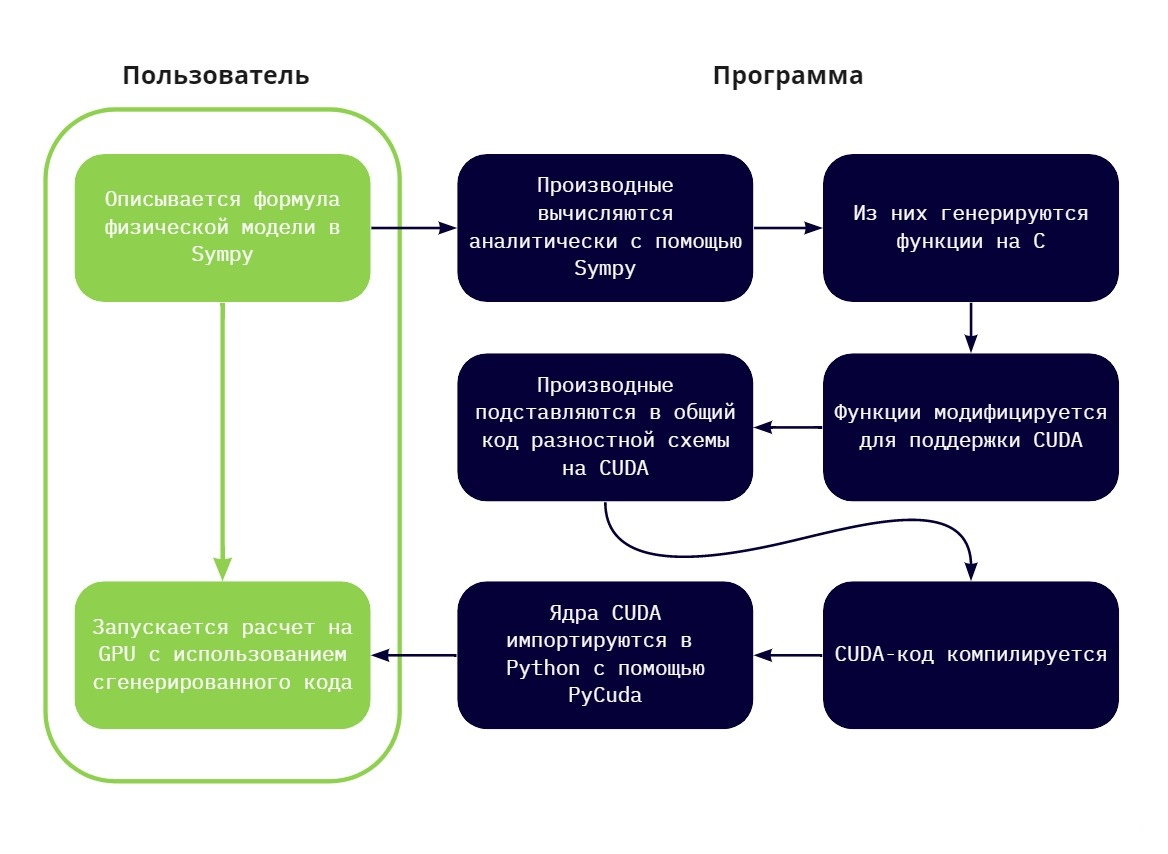
\includegraphics[width=\textwidth]{common_images/CUDA_architecture.jpg}
\caption{Архитектура программы с использованием PyCuda и Sympy}
\label{fig:cuda_architecture}
\end{figure}


\subsection{Вычисление матрицы Якоби \label{methods:computing_jacobi}}
Линейная система, которая решается в методе Ньютона, включает в себя матрицу Якоби. Рассмотрим разные подходы ее вычисления.

\subsubsection*{Прямой метод}
Можно получить явный вид матрицы Якоби: 
\begin{equation}
    J_{ij} = \frac{\partial F_i}{\partial u^n_j}
\end{equation}
Для этого нужно посчитать все частные производные аналитически. Можно делать это вручную или воспользоваться программами символьной математики, описанными в разделе \ref{implementation:symbolic}. Можно воспользоваться разреженной структурой матрицы, значительно уменьшая объем вычислений. Главный недостаток этого метода - формулы получаются очень большими.

\subsubsection*{}
Для \textit{методов подпространства Крылова} (раздел \ref{methods:linear_solvers}) достаточно знать только, как матрица действует на произвольный вектор. Сама матрица в явном виде при этом не нужна. Вместо нее мы можем создать оператор, действие которого на произвольный вектор будет давать такой же результат, как при умножении матрицы на этот вектор. Получим такой оператор:
\begin{equation}
J(x) = \frac {\partial F(x)} {\partial x}
\end{equation}
Умножение матрицы Якоби на вектор с линейной точностью равно нахождению изменению вектора $F(X)$ в направлении этого вектора:
\begin{equation}
dF(x) = J \cdot dx
\end{equation}
\begin{equation}
J \cdot a \approx dF(x) \vert_{dx = a}
\end{equation}

\subsubsection*{Разностный метод}
Вычислим $dF$ численно как производную по направлению:
\begin{equation}
dF = \frac{F(x + \varepsilon a) - F(x)}{\varepsilon}
\end{equation}
Точность такого метода настраивается выбором малого параметра $\varepsilon$. С разностным методом вычисления матрицы Якоби мы получаем метод, позволяющий решить нелинейную систему уравнений, указав только вид функции $F(x)$ для метода Ньютона. Такой метод называется \textit{JFNK-метод} (Jacobi-Free Newton-Krylov). Его свойства сходимости исследуются в \cite{JFNK}.

\subsubsection*{Аналитический метод}
Можно вычислить действие оператора Якоби, используя правило дифференцирования сложной функции. Исследуемую функцию $F$ запишем в общем виде: 
\begin{equation}
F :=L(u^n) -\varphi(u^{n-1}, x_i, t) = 0
\end{equation}
где $u^n$ - искомый вектор переменных в момент времени $t_n$, $L$ - гладкая функция, зависящая от них. В функции $\varphi$ собраны все члены, которые на зависят от неизвестного вектора $u^n$.
Дифференцируем:
\begin{equation}
dF = \frac{\partial L(u^n)} {\partial u^n} du^n
\end{equation}
Частные производные функции $L$ для конкретной задачи могут быть тоже упрощены с помощью правила дифференцирования сложных функций и вычислены с помощью символьной математики. Пример применения данного метода есть в разделе \ref{dhd:features}. Данный способ сложнее разностного метода в реализации, однако он точнее. Поэтому разностный метод можно использовать для тестирования реализации данного способа.

\subsection{Предобуславливание безматричного метода \label{implementation:operator_preconditioning}}
Численные методы решения СЛАУ используют предобуславливатели (раздел \ref{methods:preconditioning}). Для вычисления предобуславливателя нужна матрица Якоби. Но мы используем методы \textit{подпространства Крылова}, где мы не храним явный вид этой матрицы. Поэтому нужен алгоритм ее получения из безматричного представления. 
\par
Получить явный вид можно, используя результат умножения оператора Якоби на вектор $\delta^i$, у которого равны нулю все элементы, кроме $i$:
\begin{equation}
\begin{cases}
\delta^i_i = 1
\\
\delta^i_{j \neq i} = 0
\end{cases}
\end{equation}
Действие оператора Якоби на $\delta^i$ дает $i$-й столбец матрицы $J$. Для получения явного вида $J$ размерности $N \times N$ нужно сделать $N$ перемножений. 

\subsubsection*{Оптимизация вычисления}
Существует подход, позволяющий вычислить вид матрицы Якоби, подействовав оператором на вектор конечное количество раз независимо от размерности матрицы. Для этого матрица должна быть разреженной, и мы должны знать ее структуру. Рассмотрим простейший случай: пусть матрица тридиагональна \eqref{mat:tridiagonal}. Тогда $i$ строка матрицы будет влиять только на $i$, $i + 1$ и $i - 1$ элементы вектора $c$ в уравнении $A \cdot b = c$. Пусть вектор $b$ будет иметь вид:
\begin{equation}
\begin{cases}
b_i = 1, \quad i \bmod  3 = 0 \\
b_i = 0, \quad i \bmod  3 \neq 0
\end{cases}
\end{equation}
где $\bmod$ означает остаток от деления. Тогда результат умножения $c$ будет содержать в себе всю информацию о каждом третьем столбце матрицы Якоби. После этого нужно два раза повторить циклический сдвиг значений вектора $b_i$ и получить информацию о недостающих $2/3$ столбцах матрицы Якоби.

\subsubsection*{Оптимизация применения}
Пусть нам необходимо вычислить предобуславливатель на каждом шагу по времени. Тогда сводится на нет преимущество в производительности от операторного подхода, поскольку на каждом шагу мы вычисляем матрицу в явном виде.

Чтобы сохранить сильные стороны безматричного подхода, рассмотрим такую оптимизацию. Предположим, что матрица Якоби не сильно меняется от шага к шагу по времени. Тогда мы можем переиспользовать один предобуславливатель в течение нескольких следующих итераций. Поскольку это предположение никак не подкреплено теоретически, необходимо ввести параметр $P$, отвечающий за пересчет предобуславливателя. Будем пересчитывать предобуславливатель, если метод решения СЛАУ сделал больше $P$ итераций. Подбирается оптимальное значение параметра $P$, соблюдающее баланс между частым пересчетом предобуславливателя и долгой сходимостью итерационного метода. Начать расчет можно вообще без предобуславливателя. Посчитать его нужно будет, только если итерационный метод будет сходиться дольше, чем за $P$ итераций.
\par
В медленных процессах матрица Якоби действительно меняется слабо, и предобуславливатель можно переиспользовать довольно долго. Такой подход позволяет существенно сократить вычислительные затраты.

\subsection{Стратегии тестирования \label{implementation:testing}}
Реализация любого численного алгоритма - это в том числе написание программы. В ней можно допустить множество ошибок – от неправильно поставленного знака до опечатки. Поэтому важно с самого начала правильно заложить в программу стратегии тестирования. Тесты позволяют быть уверенным, что изменения внесены в алгоритм корректно и ничего не сломалось.
\par
В этой главе мы рассмотрим подходы, используемые для тестирования реализованных программ в данной работе. Некоторые из подходов реализованы в виде автоматических тестов, другие предоставляют отчет для оценки.

\paragraph{Сравнение с задачей с постоянными коэффициентами}
Если реализованы алгоритмы решения линейной и нелинейной задачи, можно сравнить их результаты, взяв нелинейный коэффициент постоянным. Рассмотрим этот тест на примере уравнения теплопроводности\eqref{eq:heat_equation_intro}. Возьмем $\alpha = const$, задача станет линейной. В случае явного метода ход решения останется таким же. Изменения в ходе решения неявного метода станут значительными. Больше не нужно решать нелинейную систему методом Ньютона (раздел \ref{methods:newton}). Остается решить систему $\mathbf{F} \cdot \mathbf{u}^{n+1} = \mathbf{b}$, где $\mathbf{F} = const$. На каждом шагу по времени нужно решить одну систему линейных уравнений. Результаты данного метода должны совпадать с результатами нелинейного алгоритма с $\alpha(u) = const$ с точностью порядка аппроксимации.

\paragraph{Тестирование операторов производной}
Оператор второй производной по пространству в коде можно выразить отдельной функцией. Тогда его будет удобно тестировать отдельно от всей задачи.
Тестирование линейной задачи проводится на полиномах и собственных функциях. 
\begin{enumerate}
\item Полиномы 1 и 2 степени должны дифференцироваться точно, так как производная по пространству аппроксимируется со 2-м порядком. Ошибка вносится только конечной машинной точностью, поэтому она увеличивается при уменьшении шага сетки. Полиномы степени $n > 2$ дифференцируются с точностью порядка аппроксимации.
\item Собственные функции под действием оператора умножаются на известное собственное значение: $D^2_x \cdot u_{eig} = \lambda \cdot u_{eig} + O(h^p)$. Собственными функциями оператора второй производной являются $sin (x)$ и $cos(x)$. 
Разность должна сходиться к нулю с порядком аппроксимации $p$: $D^2_x \cdot u_{eig} - \lambda \cdot u_{eig} = O(h^p)$
\end{enumerate}

\paragraph{Сравнение с явным методом}
Явный и неявный методы должны сходиться к одному и тому же решению с ошибкой порядка аппроксимации. Можно сравнивать решения, полученные этими методами на одной и той же сетке в одинаковый момент времени.

\paragraph{Задачи меньшей размерности}
Ход решения трехмерной задачи качественно не отличается от двумерной. Можно поставить задачу большей размерности так, что начальные, граничные условия и источник не будут зависеть от одной из координат. Тогда решаемая задача на трехмерной сетке сведется к двумерной. Мы сможем сравнить их решения. Ошибка может появиться из-за конечной машинной точности или граничных условий, однако они будут порядка аппроксимации.
\par
Данный тест позволяет сначала безошибочно реализовать одномерную задачу, потому двумерную, а затем трехмерную.

\paragraph{Кросс-валидация}
Можно сравнить результаты с другой программой, реализующей ту же самую физическую модель.

\paragraph{Проверка законов сохранения}
Если численный метод консервативный, то в нем должны выполняться законы сохранения на дискретном уровне. Например, интегральная масса в системе функционала плотности \eqref{eq:dhd_system_intro} сохраняется, если нет источников и потока через границы. На каждом шагу можно проверять закон сохранения массы: 
\begin{equation}
m = \int_{D} \rho(\mathbf{x}) d\mathbf{x}
\end{equation}

\subsubsection*{Оценка сходимости \label{implementation:convergence} }
В главе \ref{methods} были рассмотрены численные методы с порядком сходимости $O(\tau, h^2)$ или $O(\tau^2, h^2)$. Исследование сеточной сходимости позволяет оценить, насколько близок реальный порядок сходимости к теоретическому. Для этого одинаковая задача решается на разных сетках с последовательно уменьшающимся шагом. 
\par
Шаг по времени $\tau$ в исследовании сеточной сходимости нужно брать постоянным. Он делится пропорционально $h^2$, если аналитический порядок $O(\tau, h^2)$. Таким образом можно погасить вклад ошибки первого порядка по $\tau$. Если исследуется схема с порядком $O(\tau^2, h^2)$, $\tau$ делится пропорционально $h$.
\par
Рассмотрим 3 метода вычисления порядка сходимости. В случае правильной реализации задачи, все 3 покажут одинаковый порядок. Отличие в результатах может указывать на типичные ошибки в реализации.
\paragraph{Сравнение с аналитическим решением}
Численную задачу можно получить из заранее выбранной формулы - решения. Из нее вычисляются начальные и граничные условия, а также источник. После этого аналитическое решение сравнивается с численным. Это прямой метод нахождения ошибки. Его недостаток в том, что нужно вручную вычислить аналитические производные. Этот процесс можно автоматизировать с помощью символьной математики, раздел \ref{implementation:symbolic}. В результате работы данного теста формируется график зависимости нормы ошибки от шага сетки. Используется норма $L_2$ в конкретный момент времени по всему пространству. Поскольку ожидается ошибка $\varepsilon = C \cdot h^2$, график строится в логарифмическом масштабе: $\log_{10} \varepsilon = 2 \log_{10} h + \log_{10} C$. В тех же осях откладывается прямая линия $y = 2x$ для сравнения угла наклона. 
\par
Данный метод - самый точный из трех рассматриваемых, однако для его применения нужно знать аналитическое решение.

\paragraph{Порядок по мелкой сетке}
Решение на самой мелкой сетке принимается за точное решение. Другие решения сравниваются с ним. График ошибки относительно самой мелкой сетки строится на одних осях с графиком ошибки по предыдущему методу. Возможна ситуация, когда этот признак дает хороший порядок сходимости, а признак сравнения с аналитическим решением - нет. Это значит, что решения сходятся, но не к аналитическому решению. Скорее всего, допущена одна из ошибок:
\begin{itemize}
\item задача получена из аналитического решения неправильно
\item численный метод аппроксимирует другую задачу
\item решение берется не в нужных точках
\end{itemize}

\paragraph{Порядок по 3 сеткам}
Пусть $\tilde u$ - точное решение, а $u_h$ - численное решение на сетке с шагом $h$. Ищем порядок сходимости $p$, на сетках с шагом $h, \alpha h, \alpha^2 h$.
\begin{equation}
u_h = \tilde u + O(h^p) \approx \tilde u + C \cdot h^p
\end{equation}
Поэтому $|| u_h - u_{\alpha h} || \approx (1 - \alpha^p) \cdot ||C \cdot h^p||$.
\begin{equation}
\frac {||u_h - u_{\alpha h}||} {||u_{\alpha h} - u_{\alpha^p h}||} \approx \frac {1 - \alpha^p} {\alpha^p \cdot (1 - \alpha^p)} = \frac{1}{\alpha^p}
\end{equation}
Можно выразить порядок сходимости: 
\begin{equation}
p = log_\alpha \frac {||u_{\alpha h} - u_{\alpha^p h}||} {||u_h - u_{\alpha h}||}
\end{equation}
\subsection*{}
Описанные методы проверки сеточной сходимости собраны в одной программе. Она была использована для всех численных методов, реализованных в рамках данной работы. Примеры ее использования приведены в главах, посвященных конкретным задачам: \ref{heat:convergence} для уравнения теплопроводности и \ref{dhd:convergence} для системы функционала плотности.
